
\section{Methods}

In this section, we describe in detail the \emph{PPISnowball} system (Figure \ref{fig:ppisnowball}), which is an extension of snowball system\cite{Agichtein.Gravano:2000}. The workflow of \emph{PPISnowball} system is as follows:\\
(1) Document Preprocessing. (Section \ref{DocumentPreprocessing})\\
(2) Manual Selection of Positive and Negative Tuples as Seed Tuple Set.\\
(3) Extraction of Candidate Patterns. (Section \ref{GenPatterns})\\
(4) Evaluation of Patterns. (Section \ref{EvalPatterns})\\
(5) Augmentation of Candidate Patterns by Clustering and Re-Evaluation Patterns. (Section \ref{AugmentPatterns})\\
(7) Generating Candidate Tuples from Extracted Triplets. (Section \ref{GenTuples})\\
(8) Evaluation of Tuples and Adding Sufficiently-reliable Ones to to Seed Tuple Set. (Section \ref{EvalTuples})\\
(9) Repeating (3)-(8) until Converge.\\


\subsection{Document Preprocessing}
\label{DocumentPreprocessing}

\subsection{Generating Candidate Patterns}
\label{GenPatterns}

Generating patterns to find new triplets serves as a crucial step in the extraction process of \emph{PPISnowball} system. Ideally, a perfect pattern should possess two properties: \emph{selectiveness},so that they barely coincide with incorrect tuples; and high \emph{coverage},so that they are representative enough to extract many new tuples\cite{Agichtein.Gravano:2000}.

\emph{PPISnowball} initially input a set of positive example tuples, for every protein$-$protein tuple $\langle protein\_1,protein\_2\rangle$, \emph{PPISnowball} find all context in whole document collections where protein\_1,protein\_2 and at least one interaction word occur in a sentence simultaneously by consulting the dictionaries mentioned in section \ref{DocumentPreprocessing}. \emph{PPISnowball} would replace proteins and interaction word with named-entity tags before analyze that sentence on the basis of certain rules (details later) to generate patterns. Taking the following sentence(PUBMED ID:12620407) as an example, \emph{PTEN regulates the transcriptional activity of p53 by modulating its DNA binding activity}. Since "PTEN" and "p53" are protein names, "regulates" indicates the interaction relationship between them, so the sentence after tagging looks like: \emph{$\langle PROT1\rangle$ $\langle INTERACTION\rangle$ the transcriptional activity of $\langle PROT2\rangle$ by modulating its DNA binding activity}.

Generally patterns are habitual language expressions that people tend to use to elaborate their ideas, either semantically or syntactically. A sufficiently-reliable pattern is expected to occur much more often in literatures than others do. According to such belief, we implement several patterns to measure habitual usage of language to describe a PPI information, next, we will briefly introduce their design principles.\\

\textbf{Shallow Linguistic Pattern. }  The \emph{Shallow Linguistic Pattern} is solely based on surface features (capitalization, punctuation, breaker,preposition, etc.) and shallow linguistic processing features (Part-of-Speech tagging and lemmatization). We borrow the feature set defined by Chowdhary for Bayesian Network building\cite{DBLP:journals/bioinformatics/ChowdharyZL09}. There are 12 features, which are strongly related to language rules. Using previous mentioned sentence as an example, \emph{PTEN regulates the transcriptional activity of p53 by modulating its DNA binding activity}. The pattern for triplet $\langle\langle PTEN,p53\rangle,regulates\rangle$ are the following: interactor,regulates; D1,0; D2,4; order,avb; prep,NA; conditional,n; comma, nn; but,n; which,n; not,n; breaker,n and NumberOfInteractors,high.

\textbf{Tri-Branch Part-Of-Speech(POS) Tree Pattern. } The \emph{Tri-Branch Part-Of-Speech(POS) Tree Pattern} is a subtree of the syntax tree (Figure \ref{fig:postree}A) generated by Stanford Parser (http://nlp.stanford.edu/software/lex-parser.shtml). When a syntax tree is acquired, since both proteins and interaction word are located in the leaf nodes of the tree, so we can backtrack the proteins and interaction word along the branches of the syntax tree until the root, thus obtain three routine respectively, after that,we can find a minimum(lowest-level) node which serve as the common ancestor of both proteins and interaction words (Figure \ref{fig:postree}B). Regarding the minimum common ancestor node as the new root, and three routine as new branches, here we get a subtree of original syntax tree (Figure \ref{fig:postree}C). What's more, for the sake of computational efficiency and representative neatness, we remove redundant elements, for example, the node directly above the protein is bound to a noun, in forms of "NN" or "NNP", so elimination of such information would do no harm to discrimination and uniqueness of patterns. Also we exert standardization on some tags, for example, there are many variation for a single verb tag, such as "VB" for base form, "VBZ" for 3rd person singular present, "VBD" for past tense, etc.To reduce ambiguity, we replace all related variation of verb with standard "VB" (Figure \ref{fig:postree}D).

\textbf{Tri-Branch Dependency Tree Pattern. } The \emph{Tri-Branch Dependency Tree Pattern} is a subtree of the collapsed dependency tree generated by Stanford Parser. In a dependency tree, nodes stand for words from sentence, and edges stand for grammatical relationship between words (Figure \ref{fig:deptree}A). However, the dependency tree cannot be used as pattern directly, for nodes are invariably different. Compared to nodes, the dependency relationship is much more stable and common, so we reverse the edges to nodes, in addition, we keep original protein and interaction word nodes (Figure \ref{fig:deptree}B). Finally, subtree rooted at minimum common ancestor is extracted based on the similar method mentioned by \emph{Tri-Branch Part-Of-Speech(POS) Tree Pattern}. Noticing that there won't necessarily be three routines in the subtree, for the reason that interaction word might hold a dominant position and thus become the ancestor of proteins (Figure \ref{fig:deptree}C).

%\begin{flushleft}
%\begin{figure}
%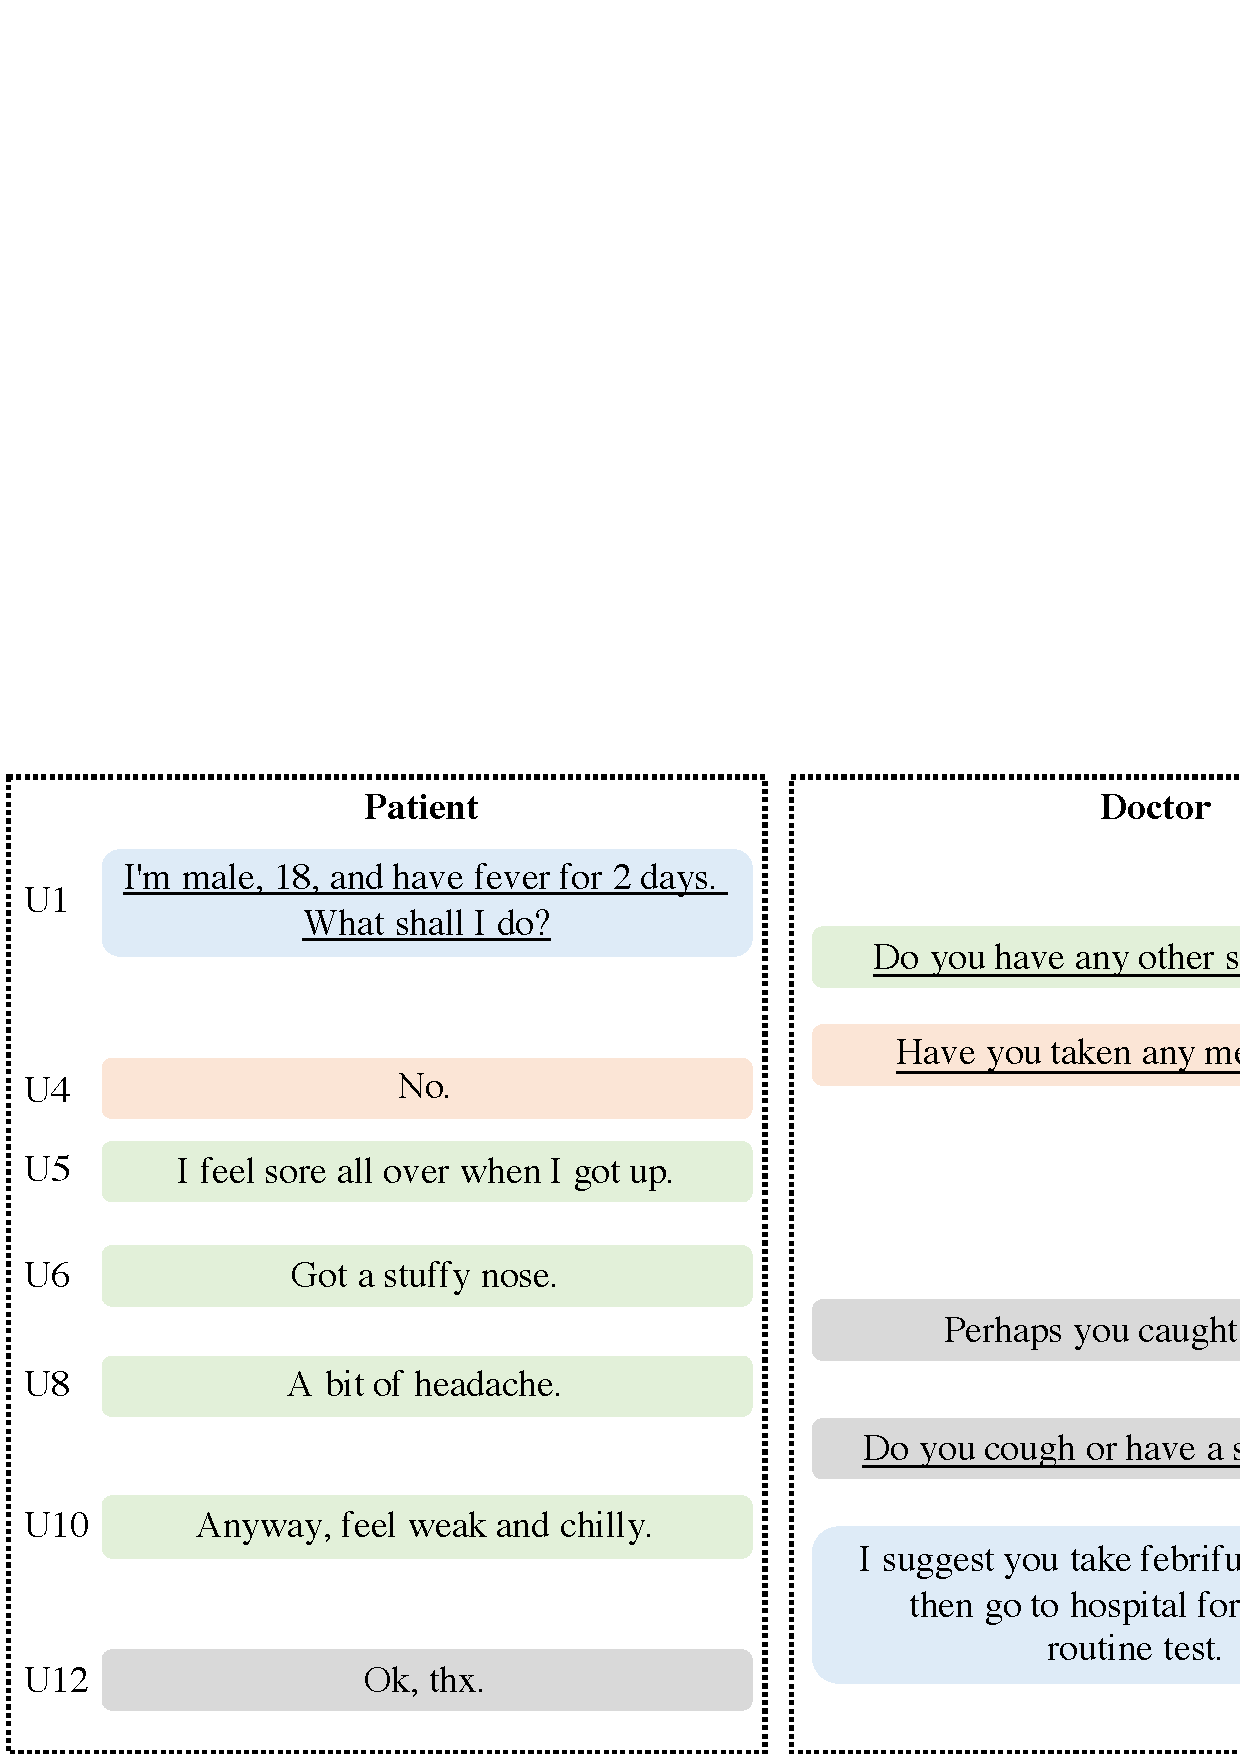
\includegraphics[width=100mm]{fig/figure3.png}
%\caption{Features used to encode protein-protein interaction rules in a sentence}
%\label{fig:feature}
%\end{figure}
%\end{flushleft}

\begin{flushleft}
\begin{figure}
\includegraphics[width=80mm]{fig/figure5.png}
\caption{How a Tri-Branch Part-Of-Speech(POS) Tree Pattern generated. The example sentence is "\emph{PTEN regulates the transcriptional activity of p53 by modulating its DNA binding activity.}" \textbf{(A)} Original syntax tree generated by Stanford parser. \textbf{(B)} Find minimum common subtree where a pair of proteins and interaction word share the same ancestor. \textbf{(C)} Extract the minimum common subtree,with only three directly related branch kept. \textbf{(D)} Remove redundant POS tags as well as do tag standardization.}
\label{fig:postree}
\end{figure}
\end{flushleft}

\begin{flushleft}
\begin{figure}
\includegraphics[width=80mm]{fig/figure6.png}
\caption{How a Tri-Branch Dependency Tree Pattern generated. The example sentence is "\emph{PTEN regulates the transcriptional activity of p53 by modulating its DNA binding activity.}" \textbf{(A)} Original dependency tree generated by Stanford parser. \textbf{(B)} Reverse the edge into nodes, in addition, keep original protein and interaction word nodes. \textbf{(C)} Prune none-directly related nodes and do tag standardization}
\label{fig:deptree}
\end{figure}
\end{flushleft}

\textbf{How to compare two distinct patterns. } In order to avoid replication of extracted patterns, a similarity function \emph{Sim(Pattern\_1,Pattern\_2)} is required to measure the distance between two patterns, of which the value belongs to [0,1]. The higher the value, the more similarity these two patterns hold. There are two kind of measure strategies, we will brief introduce their underlying principles as follows:

(1)\textbf{Rigid Similarity.} As the name implies, the rigid similarity focuses on total equality of two patterns. Either the two are exactly the same, then return 1 or they mismatch, then return 0. More specifically, for \emph{Shallow Linguistic Pattern}, only if all 12 features are identical would be regarded as the same; for \emph{Tri-Branch Part-Of-Speech(POS) Tree Pattern} or \emph{Tri-Branch Dependency Tree Pattern}, only if the extracted subtrees coincide would meet the requirement to be equal. Such all-or-nothing strategy is unsuitable to \emph{PPISnowball} system for it tends to result in low \emph{coverage}.

(2) \textbf{Soft Similarity.} Compared to rigid similarity, the soft similarity strategy is more flexible which would return a numeric number between 0 and 1. If the similarity score exceed some minimum similarity threshold $\mathcal {T}_{sim}$, then two patterns would be regarded as the same. Though seemingly promising, it still remains challenge to implement a proper soft similarity strategy. We would introduce graph kernel in detail later (Section \ref{AugmentPatterns}).




\subsection{Evaluation of Patterns}
\label{EvalPatterns}

The pattern evaluation is a key step of \emph{PPISnowball} system. "Bad" patterns might extract erroneous tuples that in turn might bring about even more "bad" patterns in the next \emph{PPISnowball} iteration. To avoid Snowball evolving into "avalanche", we expect to eliminate patterns that tends to generate wrong triplets, in other words, we prefer to highlight patterns with high selectivity. Thus, all triplets matching one specific pattern have to be taken into consideration, and put together to weigh the selectivity of that pattern.

Since a pattern is expected to occur frequently, we use a preliminary filter to eliminate patterns which is supported by less than $\mathcal {T}_{sup}$ triplets. Then, we calculate the \emph{confidence} by associating all tuples included in triplets, regardless of their current status (Positive, Negative, Unknown).\\

\textbf{Definition} The confidence of a Pattern \emph{P} is:

\begin{equation}
\begin{aligned}
&Conf(P)= \frac{W_{pos}*P.pos}{W_{pos}*P.pos + W_{neg}*P.neg + W_{unkn}*P.unkn}
\label{eq:conf}
\end{aligned}
\end{equation}

\emph{where P.pos, P.neg and P.unkn refer to the number of positive, negative and unknown triplets matching Pattern P respectively; $W_{pos}$, $W_{neg}$ and $W_{unkn}$ are the weighting coefficient correspondingly.}\\

Considering \emph{P.unknown} is highly possible to be very large, compared to initial size of positive and negative seed tuples set, the \emph{confidence} is inclined to be biased by the overlarge denominator in equation of Conf(P). To make those patterns which possess more positive triplets stand out, one alternative approach is use the \emph{RlogF confidence} derived from the evaluation of extraction patterns generated by the Autoslog-TS information system\cite{DBLP:conf/aaai/Riloff96} as follows.\\

\textbf{Definition} The RlogF confidence of a Pattern \emph{P} is:

\begin{equation}
\begin{aligned}
Conf_{RlogF}(P)=Conf(P)*\log_{2}(P.positive+1)
\end{aligned}
\end{equation}

\emph{Here we use $\log_{2}(P.positive+1)$ rather than $\log_{2}(P.positive)$ to avoid the case of zero.} \\

Finally, since the selectivity of patterns would surely deteriorate through the process of \emph{PPISnowball} iterations, we should attach importance to the pattern confidence learnt from previous iterations as well. That is to say, the final pattern confidence is the weighted average confidence between the one achieved at current iteration and the one previous iterations. To be precise, the ultimate confidence of a Pattern \emph{P} is:

\begin{equation}
\begin{aligned}
Conf(P)&=Conf_{new}(P)*W_{updt}+ \\
&Conf_{old}(P)*(1-W_{updt})
\label{eq:ultraConf}
\end{aligned}
\end{equation}

The parameter $W_{updt}$ stands for the learning rate, if $W_{updt}<0.5$, that means \emph{PPISnowball} system put higher value on old patterns or in other words, look down on new triplets extracted at current iteration.


\subsection{Augmentation Patterns}
\label{AugmentPatterns}

\subsubsection{Measurement of Pattern Similarity by Kernels.}
\label{SimKernels}

The kernel methods are a class of algorithm universally used for pattern analysis. The essence of kernel is a similarity that maps a pair of instance to a similarity score. Given a finite set of \textbf{K} instance, the kernel can be represented as a $\textbf{K}\times\textbf{K}$ similarity matrix that contains similarity scores of all pairwise combination of instances.Kernels can be computed simply by computationally-efficient inner products between the images of all pairs of instance, rather than make operation in a much higher dimension of feature spaces such as graphs or trees.

\textbf{Rigid Kernel.} Without loss of completeness and uniformity, we include the case of rigid similarity here by implementing a rigid kernel. According to the definition of rigid similarity (Section \ref{GenPatterns}), The similarity matrix of rigid kernel is a diagonal matrix, that is, elements are equal to one in diagonal and zero for the rest. To be precise, the rigid kernel function \emph{$K_{rigid}$(Pattern\_i,Pattern\_j)} between two pattern is defined as:

\begin{equation}
\begin{aligned}
K_{rigid}(Pattern\_i,Pattern\_j) =
\begin{cases}
 1 & \text{ if } i=j \\
 0 & \text{ if } i\neq j
\end{cases}
\end{aligned}
\end{equation}

\textbf{Shallow Linguistic Kernel. } We define \emph{Shallow Linguistic Kernel} specifically for \emph{Shallow Linguistic Pattern}. Since most of the features defined are incomparable, or at least, difficult for quantification, for example, you cannot tell too hastily the extent to which a pattern \emph{P} with a preposition is different from the pattern without. So we only take into consideration D1 value(number of words between first two elements of a triplet) and D2 value (number of words between last two elements of a triplet) for similarity comparison. Here we borrow the idea of edit distance, to be precise, the shallow linguistic function \emph{$K_{SL}$(Pattern\_i,Pattern\_j)} between two pattern is defined as:

\begin{equation}
\begin{aligned}
K_{SL}(Pattern\_i,Pattern\_j) &= \\
&\begin{cases}
 e^{-\gamma (\triangle D1 + \triangle D2)} & \text{ if } SameOrder \\
 0 & \text{ if } otherwise
\end{cases}
\end{aligned}
\end{equation}

\emph{$\triangle$D1,$\triangle$D2 is the absolute value of D1,D2 difference between $Pattern\_i$,$Pattern\_j$; SameOrder indicates the PPI orders of $Pattern\_i$ and $Pattern\_j$ are identical.} \\

\textbf{Subtree Kernel(ST).} The \emph{subtree kernel} quantify the similarity of two trees through counting all common subtrees\cite{DBLP:conf/nips/ViswanathanS02} (Figure \ref{fig:convKernel}A) in the Tri-Branch Tree representation generated at section \ref{GenPatterns}. Only if the node labels, subtrees and their order are identical would be two trees regarded as the same.

\textbf{Subset Tree Kernel(SST).} The \emph{subset tree kernel} is quite similar to \emph{subtree kernel}, except that it is no longer bound to the restriction that all descendants have to be included in the substructures\cite{DBLP:conf/nips/CollinsD01}. Given a tree node, either none or all of its descendants need to be included in the subset tree (Figure \ref{fig:convKernel}C).

\textbf{Spectrum Tree Kernel(SpT)\cite{Kuboyama07}.} The \emph{spectrum tree kernel} focuses on directed motifs with certain size \emph{k}, called \emph{k-gram}, rather than subtrees\cite{DBLP:conf/nips/CollinsD01} (Figure \ref{fig:convKernel}B). A \emph{spectrum tree} is represented by a set of \emph{k-grams}, usually \emph{k} is 3 or 4. Noticing that the edges are directed, that is, a$\longrightarrow$b$\longrightarrow$c is different from a$\longrightarrow$b$\longleftarrow$c. \\

\begin{figure*}[htb]
\centering
\includegraphics[width=1.0\textwidth]{fig/figure7.png}
\caption{Kernels}
\label{fig:convKernel}
\end{figure*}

After a similarity matrix is defined by kernel functions, for a query pattern, the simplest and most natural choice is to find \emph{k} nearest neighbor patterns by looking after those patterns with highest similarity scores; Alternatively, we could find out all those patterns of which the similarity scores exceed some minimum similarity threshold $\mathcal {T}_{sim}$. Finally, we add new patterns associated with similarity to the candidate pattern sets for further evaluation.

\subsubsection{Evaluation of Augmented Patterns}
The evaluation of those augmented patterns is crucial, for the reasons that additional qualified patterns would transcend the limited size and narrow coverage of original candidate pattern set and thus contribute to the diversity of results of tuple extraction at last; on the other hand, if those "bad" patterns escape from filtering and play the role of extracting new tuples, then performance would be jeopardized, what's even worse, less satisfactory than the situation without applying pattern augmentation.

The confidence of an augmented pattern is twofold: first, according to the essence of pattern evaluation (Section \ref{EvalPatterns}), all triplets matching one specific pattern are put together to contribute to the confidence of certain pattern; second, since the augmented patterns are achieved due to an original one by similarity, so their confidences should be highly related to the confidence of original pattern in some sense. Also, chances are high that an newly-augmented pattern already exists actually, in that case, the confidence of that pattern should be enhanced for its validity is proved by similar counterparts. Finally, we believe augmented patterns less than those directly generated by seed tuples, so we downgrade the importance of augmented patterns to some extent. Consider an augmented Pattern \emph{$P_{aug}$}, and it is induced by original Pattern \emph{$P_{origin}$} based on similarity \emph{sim}, then we calculate the confidence of the augmented Pattern \emph{$P_{aug}$} based on algorithm \emph{CALCULATE-AUGPATTERN-CONF}:

%\begin{equation}
%\begin{aligned}
%Conf_{aug}(P_{aug})&=\bbbeta *(W_{own}*Conf(P_{aug}) \\
%        &+ (1-W_{own})*sim*Conf(P_{origin}))
%\end{aligned}
%\end{equation}

\begin{codebox}
\Procname{$\proc{Calculate-AugPattern-Conf($P_{aug}, P_{origin}, sim$)}$}
\li $conf \gets 0$
\li \If $P_{aug}$ already exists
\li     \Then
            $conf \gets Conf(P_{aug})$
        \End
\li $newConf \gets \bbbeta *(W_{own}*Conf(P_{aug})$\zi \space\space\space\space\space\space\space $+(1-W_{own})*sim*Conf(P_{origin}))$
\li $conf \gets conf+newConf$
\li \Return $conf$
\end{codebox}

The parameter $W_{own}$ represents for the augmentation rate. If $W_{own}>0.5$ then the \emph{PPISnowball} system in effect trusts more in the own confidence brought from corresponding triplets, shown as $Conf(P_{aug})$, which will lead to more independent patterns and have a diversified effect; else if $W_{own}<0.5$ then the \emph{PPISnowball} system appears to trusts more in the derived confidence resulting from similarity associations, shown as $sim*Conf(P_{origin})$, which will lead to more interdependent patterns and have a clustering effect. For our experiments, we set $W_{own}=0.5$. Besides, the parameter $\bbbeta$ is a numeric number, ranging from 0 to 1. It downgrades the importance of augmented patterns in terms of confidence. If a newly-augmented pattern already exists, the confidence would be accumulated.




\subsection{Generating Candidate Tuples}
\label{GenTuples}

After candidate patterns are generated and evaluated, \emph{PPISnowball} system scans whole documents set to discover new triplets. Initially, \emph{PPISnowball} identify all sentences which possess at least two different proteins and at least one interaction words. If there are \emph{n (n$\geq$2)} proteins and \emph{k (k$\geq$1)} interaction words are spotted in a sentence, then the number of total possible candidate triplets is $\left(\begin{smallmatrix} n\\2 \end{smallmatrix} \right)$)*k. For each possible candidate triplet $\langle\langle protein\_1,protein\_2\rangle,interaction\rangle$, we generate its pattern \emph{P} based on the surrounding context in the sentence. If the pattern \emph{P} exactly hits the candidate patterns set, the tuple within that triplet is accepted for further evaluation in next step.


\subsection{Evaluation of Tuples}
\label{EvalTuples}

%After candidate tuples are extracted by patterns, \emph{PPISnowball} use two totally different approaches to evaluate the quality of each tuple. Next, we will briefly introduce their evaluation principles as follows:\\

Since each tuple can be generated from a number of patterns, that is to say, to quantify the goodness of a certain tuple involves associating with confidences of those patterns. Consider a candidate tuple \emph{T} and a set of patterns \emph{P=\{$P_{i}$\}} that generate such tuple \emph{T}. Assuming for the moment we have already calculated confidence score for each pattern $P_{i}$, called \emph{Conf($P_{i}$)}, then we define the confidence of candidate tuple \emph{T} to be:

\begin{equation}
\begin{aligned}
Conf(T)=1-\prod_{i=0}^{|P|}(1-Conf(P_{i})))
\end{aligned}
\end{equation}

\emph{where P=\{$P_{i}$\} is the set of patterns that facilitate generating tuple \emph{T}}\\

%(2) There is an assumption that a valid tuple of proteins, which possesses an interaction between each other, are biologically related tightly. Based on that, we calculate the biological distance between two proteins directly by mapping proteins to Gene Ontology(GO) (http://www.geneontology.org).The GO project provides an ontology of defined terms representing gene product properties and is structured as a directed acyclic graph\cite{geneontology04}. Therefore the PPI relationship can be somewhat validated by the closeness of distance between two proteins in that directed acyclic graph. Here we use GoSim package (http://cran.r-project.org/web/packages/GOSim/index.html).This package implements several functions useful for computing similarities between GO terms and gene products based on their GO annotation \cite{DBLP:journals/bmcbi/FrohlichSPB07}. The value of similarity is between 0 and 1, we can regard it as sort of confidence.

After calculating the confidence of candidate tuples, \emph{PPISnowball} discards all tuples with low confidence. Just like the negative effect of wrong patterns, those tuples with low confidence might cause \emph{PPISnowball} system to extract erroneous patterns in next iteration and in turn generate more "bad" tuples, resulting in the deterioration of the performance of \emph{PPISnowball} system. So we throw away tuples of which the confidence value is below some prespecified threshold $\mathcal {T}_{t}$, after that, we add the remaining survivors to seed positive tuples for next iteration.







